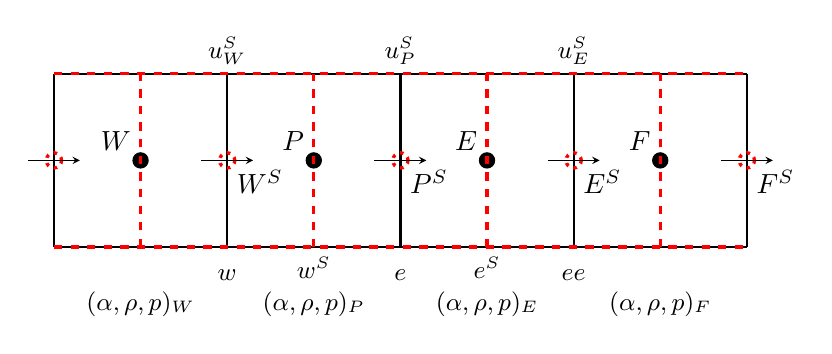
\begin{tikzpicture}[scale=1.1, >=stealth]




% Maillage primaire

% Lignes
\draw[thick] (3, 2) -- (11, 2);
\draw[thick] (3, 0) -- (11, 0);

\draw[thick] (3, 0) -- (3, 2);
\draw[thick] (5, 0) -- (5, 2);
\draw[thick] (7, 0) -- (7, 2);
\draw[thick] (9, 0) -- (9, 2);
\draw[thick] (11, 0) -- (11, 2);


% Nœuds
\filldraw (4, 1) circle  (2.5pt);
\node[above left] at (4, 1) {\(W\)};

\filldraw (6, 1) circle  (2.5pt);
\node[above left] at (6, 1) {\(P\)};

\filldraw (8, 1) circle  (2.5pt);
\node[above left] at (8, 1) {\(E\)};

\filldraw (10, 1) circle  (2.5pt);
\node[above left] at (10, 1) {\(F\)};

% Bords
\node[below] at (5, -0.15) {\small \(w\)};
\node[below] at (7, -0.15) {\small \(e\)};
\node[below] at (9, -0.15) {\small \(ee\)};

% Variables
\node[below] at (4, -0.4) {\small \( ( \alpha, \rho, p)_{W} \) };
\node[below] at (6, -0.4) {\small \( ( \alpha, \rho, p)_{P} \) };
\node[below] at (8, -0.4) {\small \( ( \alpha, \rho, p)_{E} \) };
\node[below] at (10, -0.4) {\small \( ( \alpha, \rho, p)_{F} \) };

% Maillage dual

% Lignes
\draw[dashed, red, very thick] (3, 2) -- (11, 2);
\draw[dashed, red, very thick] (3, 0) -- (11, 0);

\draw[dashed, red, very thick] (4, 0) -- (4, 2);
\draw[dashed, red, very thick] (6, 0) -- (6, 2);
\draw[dashed, red, very thick] (8, 0) -- (8, 2);
\draw[dashed, red, very thick] (10, 0) -- (10, 2);

% Nœuds
\draw[dotted, red, very thick] (3, 1) circle (2.5pt);

\draw[dotted, red, very thick] (5, 1) circle (2.5pt);
\node[below right] at (5, 1) {\(W^S\)};

\draw[dotted, red, very thick] (7, 1) circle (2.5pt);
\node[below right] at (7, 1) {\(P^S\)};

\draw[dotted, red, very thick] (9, 1) circle (2.5pt);
\node[below right] at (9, 1) {\(E^S\)};

\draw[dotted, red, very thick] (11, 1) circle (2.5pt);
\node[below right] at (11, 1) {\(F^S\)};

% Bords
\node[below] at (6, 0) {\small \(w^S\)};
\node[below] at (8, 0) {\small \(e^S\)};

% Variables
\node[above] at (5, 2) {\small \(u_W^S\)};
\node[above] at (7, 2) {\small \(u_P^S\)};
\node[above] at (9, 2) {\small \(u_E^S\)};

% Flux 
\draw[->, very thin] (2.7, 1) -- (3.3, 1);
\draw[->, very thin] (4.7, 1) -- (5.3, 1);
\draw[->, very thin] (6.7, 1) -- (7.3, 1);
\draw[->, very thin] (8.7, 1) -- (9.3, 1);
\draw[->, very thin] (10.7, 1) -- (11.3, 1);



\end{tikzpicture}